% https://web.njit.edu/~vitaly/121/notes121.pdf
\part{Electromagnetic Fields}
\chapter{Electric Fields}
\section{Direct-Current Circuits}
\subsection{Electric Current and Resistance}
\subsubsection{Current}
The unit of current is defined in terms of the attractive force between two currents flowing in a parallel direction. Suppose the attractive force acting between two identical straight, parallel currents located one meter apart from each other is $2 \times 10^{-7}$ N for every meter of wire. Then, we define the amount of this current to be 1 A (ampere). 

An electric current of 1 A carries an electric charge of 1 C (coulomb) in 1 s. 

\subsubsection{Potential difference}
When the energy needed to carry an electric charge of 1 C against a potential difference (also called voltage) is 1 J (joule), this potential difference is defined to have a value of 1 V (volt).

\subsubsection{Resistance}
 When a voltage of 1 V is applied to a conductor, and a current
of 1 A flows in the conductor, the electric resistance of the conductor is defined to have a value of 1 $\Sigma$ (ohm).

The resistance of a conductor $R$ is defined in terms of the voltage applied to the conductor $V$ and the current flowing in the conductor $I$ as $R \equiv \dfrac{V}{I}$. This relation can be expressed as
\begin{equation}
{V=IR
}\end{equation}

\subsubsection{Ohm's Law}
\begin{thrm}{Ohm's Law}{}
When the resistance of the conductor $R$ is independent of the applied voltage $V$ or current $I$, the conductor satisfies \textbf{Ohm’s law}.

Such a resistance is called an \textbf{ohmic resistance}. The resistance of some conductors varies with voltage or current, and such a resistance is called a non-ohmic resistance.
\end{thrm}

\subsubsection{Resistivity}
The resistance of a conductor $R$ is proportional to its length $l$ and
inversely proportional to its cross-sectional area $A$:
\begin{equation}
{R = \rho \frac{l}{A}
}\end{equation}

where $\rho$ is the resistivity of the conductor, the value of which depends on the material and its temperature.

\subsection{Kirchhoff’s Rules}
\begin{thrm}{Kirchhoff ’s junction rule}{}
At any junction in an electric circuit, sum of the currents flowing into and out of that junction are equal.
\begin{equation}
\sum I_\text{in} = \sum I_\text{out}
\end{equation}
\end{thrm}

\begin{proof}
This rule implies the conservation of charge.
\end{proof}

The influence that makes a current flow from a lower to a higher potential is called an electromotive force (emf).

\begin{thrm}{Kirchhoff’s loop rule}{}
In any closed loop of an electric circuit, sum of all the electric potential differences around a loop is zero.
\[ \sum \Delta V = 0 \]
\end{thrm}
\pagebreak

\section{Electrostatics}
\subsection{Charge}
Charge carriers are protons and electrons, where protons have a positive charge $+e$ and electrons have a negative charge $-e$.

$e$ is the fundamental charge, $e=1.60\times10^{-19}$ \unit{C}.

Charge is quantised; it comes in discrete quantities in intervals of the fundamental charge.
\[ Q=ne \]
where $n$ is an integer number of excess positive or negative charges on the object.

\subsection{Electric force and field}
In an \textbf{electric field}, an \textbf{electric force} is exerted on a charged object placed in the field.

\begin{figure}[H]
    \centering
    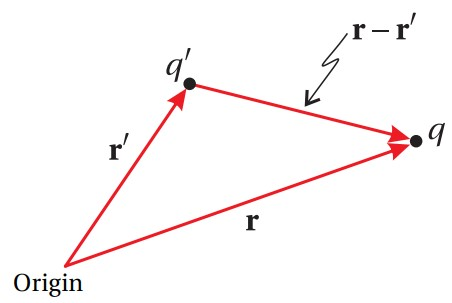
\includegraphics[width=7cm]{images/coulomb_law.jpg}
\end{figure}

The force on a point charge $q$ located at $\vb{r}$ exerted by another point charge $\vb{q}^\prime$ located at $\vb{r}^\prime$ is
\begin{equation}
{\vb{F} = q\vb{E}(\vb{r})
}\end{equation}
where
\begin{equation}
{\vb{E}(\vb{r}) = \frac{q^\prime}{4\pi\varepsilon_0} \frac{\vb{r}-\vb{r}^\prime}{|\vb{r}-\vb{r}^\prime|^3}
}\end{equation}
This relationship is known as \textbf{Coulomb’s law}. The force is directed along the vector $\vb{r}-\vb{r}^\prime$, which points from charge $q^\prime$ to $q$. 
The familiar inverse square law can be seen by noting that $\dfrac{\vb{r}-\vb{r}^\prime}{|\vb{r}-\vb{r}^\prime|}$ is a unit vector.

\begin{thrm}{Coulomb's law}{}
Consider the electric field produced by a point charge in vacuum. When a point test charge $q$ is located at a distance $r$ from a point source charge $Q$, the electric force that two charges $q$ and $Q$ exert on each other is
\begin{equation}
{\vb{F} = \frac{Qq}{r^2}
}\end{equation}
where $\varepsilon_0$ is the permittivity of vacuum.
\end{thrm}

Dividing both sides of the above equation by $q$ gives us electric field strength $\vb{E}$:
\begin{equation}
{\vb{E} = \frac{1}{4\pi\varepsilon_0}\frac{Q}{r^2}
}\end{equation}

We use electric field lines to visualise an electric field. An electric field line is a curve or line whose tangent at point gives the direction of the electric field vector $\vb{E}$ at that point. The number of electric field lines through a unit area perpendicular to $\vb{E}$ is equal to the magnitude of $\vb{E}$. Electric field lines are directed away from positive to negative charges, never intersect one another, and are never created nor annihilated in vacuum.

\subsection{Electric potential and energy}
Electric force is a conservative force. Work done by electric force on charge $q$ when the charge moves from position A to position B does not depend on the path taken.

Since work done by electric force only depends on the location of the initial (A) and final (B) positions, we can define an electrical potential energy function $U(r)$ that depends on position $r$. Work done by electric force $F_E$ on a charge in going from position A (defined by position vector, $r_A$) to position B (defined by position vector $r_B$) can be written as:
\[ W = \int_A^B \vb{F}_E \cdot \dd{\vb{r}} = -\Delta U = -\sqbrac{U(r_B)-U(r_A)} \]
Work done by electric force when $q$ moves from A to B is given by
\[ W = \int_A^B F_E\cdot\dd{r} = \int_{r_A}^{r_B} k\frac{Qq}{r^2} \dd{r} = kQq \int_{r_A}^{r_B} \frac{1}{r^2} \dd{r} = kQq\sqbrac{-\frac{1}{r}}_{r_A}^{r_B} = -\brac{\frac{kQq}{r_B} - \frac{kQq}{r_A}} \]

Hence electric potential energy is
\begin{equation}
U = \frac{1}{4\pi\epsilon_0}\frac{Qq}{r}
\end{equation}

Electric potential is the electric potential energy per unit charge, given by
\begin{equation}
V=\frac{1}{4\pi\varepsilon_0}\frac{Q}{r}
\end{equation}

\subsection{Continuous charge distribution}
A system of charges can be modelled as a \textbf{continuous charge distribution} when the electric field strength or electric potential due to the system is to be computed at a point much further than the distance between charges within the system.

Electric field strength or electric potential due to a continuous charge distribution is evaluated for each \textbf{infinitesimally small charge element}.

Electric field strength at a point due to charge element $\dd{q}$:
\[ \dd{\vb{E}} = \frac{\dd{q}}{4\pi\varepsilon_0r^2}\hat{\vb{r}} \]

Electric potential due to $\dd{q}$:
\[ \dd{V} = \frac{\dd{q}}{4\pi\varepsilon_0r} \]

Hence total electric field strength due to continuous charge distribution is 
\begin{equation}
\vb{E} = \frac{1}{4\pi\varepsilon_0} \int \frac{\dd{q}}{r^2} \hat{\vb{r}}
\end{equation}

and total electric potential is
\begin{equation}
V = \frac{1}{4\pi\varepsilon_0} \int \frac{\dd{q}}{r}
\end{equation}

The concept of \textbf{charge density} can be utilised most of the time for uniform charge distribution:
\begin{itemize}
\item \textbf{Linear charge density} $\lambda$ (charge uniformly distributed along line):
\[ \lambda = \frac{Q}{L} \]
\item \textbf{Surface charge density} $\sigma$ (charge uniformly distributed on surface):
\[ \sigma = \frac{Q}{A} \]
\item \textbf{Volume charge density} $\rho$ (charge uniformly distributed on volume):
\[ \rho = \frac{Q}{V} \]
\end{itemize}

These can be summarised as
\begin{equation*}
\dd{q} = \begin{cases}
    \lambda\dd{A} & \text{linear distribution} \\
    \sigma\dd{A} & \text{surface (area) distribution} \\
    \rho\dd{V} & \text{volume distribution} \\
\end{cases}
\end{equation*}
\pagebreak

Electric Field on the Axis of a Rod:
\begin{exmp}
A rod of length $L$ has a uniform positive charge per unit length $\lambda$ and a total charge $Q$. 

Calculate the electric field strength and the electric potential at a point $P$ that is located along the long axis of the rod and is a distance $a$ from one end.
\end{exmp}

%\begin{figure}[H]
%\centering
%\begin{tikzpicture}
%    \draw[-to] (-3,0) -- (10,0) \node [right] {$x$};
%    \draw[-to] (0,-3) -- (0,6) \node [above] {$y$};
%\end{tikzpicture}
%\end{figure}

\begin{proof}[Solution]
Set up coordinate system: rod lies on $x$-axis, point $P$ lies on origin at a distance $a$ from rod.

The electric field strength $\dd{\vb{E}}$ at $P$ due to charge element $\dd{q}$ is in the negative $x$ direction, since each charge element carries a positive charge.

Using linear charge density,
\[ \lambda = \frac{Q}{L} = \odv{q}{x} \implies \dd{q}=\lambda\dd{x} \]

Electric field strength at $P$ due to element $\dd{x}$ at a distance $x$ from $P$ is 
\[ \dd{\vb{E}} = \frac{\dd{q}}{4\pi\varepsilon_0x^2} = \frac{\lambda\dd{x}}{4\pi\varepsilon_0x^2} \]
Hence total electric field strength at $P$ is
\[ \vb{E} = \int \dd{\vb{E}} = \int_a^{L+a}\frac{\lambda\dd{x}}{4\pi\varepsilon_0x^2} = \boxed{\frac{Q}{4\pi\varepsilon_0a(L+a)}} \]

Similarly, electric potential at $P$ due to element $\dd{x}$ is 
\[ \dd{V} = \frac{\dd{q}}{4\pi\varepsilon_0x} = \frac{\lambda\dd{x}}{4\pi\varepsilon_0x} \]
Hence total electric potential at $P$ is
\[ V = \int \dd{V} = \int_a^{L+a} \frac{\lambda\dd{x}}{4\pi\varepsilon_0x} = \boxed{\frac{Q}{4\pi\varepsilon_0}\ln\brac{\frac{L+a}{a}}} \]

The answers can be verified by checking if $E=-\odv{V}{a}$ is valid.
\end{proof}
\pagebreak

Electric Field on the Axis of a Ring:
\begin{exmp}
A ring of radius $a$ carries a uniformly distributed positive total charge $Q$. 

Calculate electric field strength and electric potential at a point $P$ lying a distance $x$ from its centre along the central axis perpendicular to the plane of the ring.

Hence determine the positions where the magnitude of electric field strength is maximum.
\end{exmp}

\begin{proof}[Solution]
Electric field strength $\dd{\vb{E}}$ at $P$ due to charge element $\dd{q}$ can br resolved into components
\begin{itemize}
\item $\dd{\vb{E}}_x$ parallel to the axis of the ring
\item $\dd{\vb{E}}_y$ perpendicular to the axis.
\end{itemize}
For charge elements on opoisite sides of the ring, $\dd{\vb{E}}_y$ cancel out, so we only need to consider parallel components $\dd{\vb{E}}_x$.

Let $\theta$ be the angle between axis of ring and line joining $\dd{q}$ and $P$. Then
\[ \dd{\vb{E}}_x = \dd{\vb{E}}\cos\theta \]

Electric field strength at $P$ (at a distance $r$, perpendicular distance $x$ from ring) due to element $\dd{q}$ is
\[ \dd{\vb{E}} = \frac{\dd{q}}{4\pi\varepsilon_0r^2}\cos\theta = \frac{x\dd{q}}{4\pi\varepsilon_0(a^2+x^2)^\frac{3}{2}} \]
since $\cos\theta=\dfrac{x}{r}$ and $r=\sqrt{a^2+x^2}$.

Since all elements make the same contribution to the field at $P$ as they are all equidistant from this point, total electric field strength at $P$ is
\[ \vb{E} = \int \dd{\vb{E}} = \int \frac{x\dd{q}}{4\pi\varepsilon_0(a^2+x^2)^\frac{3}{2}} = \boxed{\frac{Qx}{4\pi\varepsilon_0(a^2+x^2)^\frac{3}{2}}} \]

Electric potential at $P$ due to element $\dd{q}$ is
\[ \dd{V} = \frac{\dd{q}}{4\pi\varepsilon_0r} = \frac{\dd{q}}{4\pi\varepsilon_0(a^2+x^2)^\frac{1}{2}} \]
Hence total electric potential at $P$ is
\[ V = \int\dd{V} = \int \frac{\dd{q}}{4\pi\varepsilon_0(a^2+x^2)^\frac{1}{2}} = \boxed{\frac{Q}{4\pi\varepsilon_0(a^2+x^2)^\frac{1}{2}}} \]

To evaluate position where $\vb{E}$ is maximum,
\[ \odv{\vb{E}}{x} = \frac{Q}{4\pi\epsilon_0}\sqbrac{\frac{a^2-2x^2}{(a^2+x^2)^\frac{5}{2}}} = 0 \implies \boxed{x=\pm\frac{a}{\sqrt{2}}} \]
\end{proof}
\pagebreak

Electric Field Due to a Uniformly Charged Disk:
\begin{exmp}
A disk of radius $R$ has a uniform surface charge density $\sigma$.

Calculate the electric field strength and electric potential at a point $P$ lying a distance $x$ from its centre along the central axis perpendicular to the disc.

Hence derive the electric field strength of an infinite, uniformly charged plate.
\end{exmp}

\begin{proof}[Solution]
A disk can be considered to be a set of concentric rings with diameter $r$ and thickness $\dd{r}$. Since surface charge density $\sigma=\frac{Q}{A}=\frac{dq}{dA}$, charge of one ring is
\[ \dd{q} = \sigma\dd{A} = \sigma\cdot2\pi\dd{r} \]
so the parallel electric field strength at $P$ due to this ring is 
\[ \dd{E} = \frac{x\dd{q}}{4\pi\varepsilon_0(r^2+x^2)^\frac{3}{2}} = \frac{\sigma rx\dd{r}}{2\varepsilon_0(r^2+x^2)^\frac{3}{2}} \]
Hence total electric field strength at $P$ is
\[ E = \int\dd{E} = \frac{\sigma x}{2\epsilon_0} \int_0^R\frac{r\dd{r}}{(r^2+x^2)^\frac{3}{2}} = \frac{\sigma x}{2\epsilon_0} \sqbrac{-\frac{1}{(r^2+x^2)^\frac{1}{2}}}_0^R = \boxed{\frac{\sigma}{2\varepsilon_0}\sqbrac{1-\frac{x}{(R^2+x^2)^\frac{1}{2}}}} \]

Similarly, electric potential at $P$ due to the ring is 
\[ \dd{V} = \frac{\sigma r\dd{r}}{2\varepsilon_0(r^2+x^2)^\frac{1}{2}} \]
Hence total electric potential at $P$ is
\[ V = \int\dd{V} = \frac{\sigma}{2\varepsilon_0}\int_0^R\frac{r\dd{r}}{(r^2+x^2)^\frac{1}{2}} = \frac{\sigma}{2\varepsilon_0}\sqbrac{(r^2+x^2)^\frac{1}{2}}_0^R = \boxed{\frac{\sigma}{2\varepsilon_0}\sqbrac{(R^2+x^2)^\frac{1}{2}-x}} \]

For an infinite, uniformly charged plate, $R\to\infty$ thus
\[ \boxed{E = \frac{\sigma}{2\varepsilon_0}} \]
\end{proof}
\pagebreak

\section{Electric flux}
\begin{defn}{Electric flux}{}
Product of electric field strength $\vb{E}$ and component of area perpendicular to the field.
\begin{equation}
{\Phi_E \equiv \vb{E} \cdot \vb{A} = EA\cos\theta
}\end{equation}
where $\theta$ is the angle between $\vb{E}$ and $\vb{A}$.
\end{defn}

\begin{figure}[H]
    \centering
    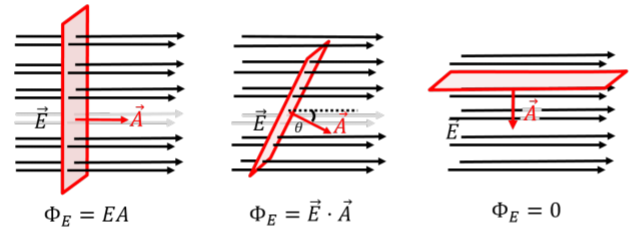
\includegraphics[width=12cm]{images/eflux.png}
\end{figure}

In cases where electric field is not uniform, we need to use the integral equation for electric flux:
\[ \dd{\Phi}_E = \vb{E}\cdot\dd{\vb{A}} \implies \Phi_E = \int \dd{\Phi_E} = \int \vb{E} \dd{\vb{A}} \]
where $\dd{\vb{A}}$ is the area vector perpendicular to the infinitesimally small surface, $\theta$ is the angle between $\vb{E}$ and $\dd{\vb{A}}$.

Total electric flux over any surface area is thus
\[ \Phi_E = \int_\text{surface}\vb{E}\cdot\dd{\vb{A}} \]

Typically total electric flux is evaluated over a closed surface. In such cases we replace the integral by
\begin{equation}
{\Phi_E \equiv \oint\vb{E}\cdot\dd{\vb{A}} = \oint E_n\dd{A}
}\end{equation}
where $E_n$ is the component of electric field strength normal to the surface.
\pagebreak

\begin{exmp}
Calculate the total electric flux through a spherical surface of radius $r$ with a charge $q$ located at its centre.
\end{exmp}

\begin{proof}[Solution]
Electric field strength at a distance $r$ from charge $q$ is
\[ \vb{E} = \frac{q}{4\pi\varepsilon_0r^2}\hat{\vb{r}} \]

Hence total electric flux is
\[ \Phi_E = \oint\frac{q}{4\pi\varepsilon_0r^2}\hat{\vb{r}}\cdot\dd{A} = \oint\frac{q}{4\pi\varepsilon_0r^2}\cdot\dd{A} = \frac{q}{4\pi\varepsilon_0r^2}4\pi r^2 = \frac{q}{\varepsilon_0} \]
\end{proof}
\pagebreak

\section{Gauss's Law}
For a point charge $q$ located at the centre of a sphere of radius $r$, magnitude of electric field everywhere on the surface of sphere is $\dfrac{k_eq}{r^2}$. We call the closed surface of the sphere a \textbf{gaussian surface} and the net electric flux through this surface is
\[ \Phi_E = \oint\vb{E}\cdot\dd{\vb{A}} = E\oint\dd{\vb{A}} \]
Using the expression for electric field and surface area of sphere, net flux through gaussian surface is 
\[ \Phi_E = \frac{q}{4\pi\varepsilon_0r^2}4\pi r^2 = \frac{q}{\varepsilon_0} \]

\begin{remark}
Net flux through any closed surface surrounding a point charge is independent of shape of that surface.

Net flux through a closed surface that surrounds no charge is zero.

Electric field due to many charges is the vector sum of electric fields produced by the individual charges.
\[ \oint\vb{E}\cdot\dd{\vb{A}} = \oint(\vb{E}_1+\vb{E}_2+\cdots)\cdot\dd{\vb{A}} \]
\end{remark}

Formally, 
\begin{thrm}{Gauss's Law}{}
Net flux through any closed surface surrounding a point charge $q$ is given by $\dfrac{q}{\varepsilon_0}$ and is independent of the shape of the surface.
\begin{equation}
{\Phi_E = \oint\vb{E}\cdot\dd{\vb{A}} = \frac{q_\text{in}}{\varepsilon_0}
}\end{equation}
\end{thrm}

\begin{figure}[H]
    \centering
    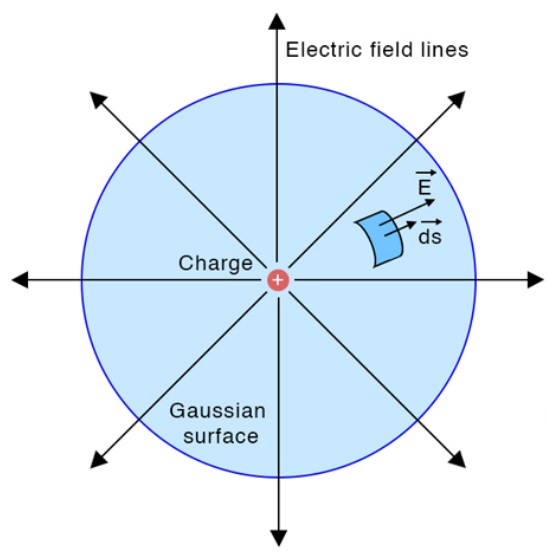
\includegraphics[width=8cm]{images/gauss_law_e.jpg}
\end{figure}

Conditions for Gauss's Law
\begin{itemize}
\item The surface must be closed.
\item The surface must pass through the point where the electric field is calculated.
\item The charge must be inside the surface.
\item The charge distribution must be continuous. The law cannot be applied to discrete charges.
\end{itemize}

Coulomb's Law derived from Gauss's Law:
\begin{proof}[Derivation]
Electric flux is given by
\[ \Phi_E = \oint\vb{E}\cdot\dd{\vb{A}} \]
If $\vb{E}$ and $\dd{\vb{A}}$ are parallel everywhere on the surface,
\[ \oint\vb{E}\cdot\dd{\vb{A}} = \oint E \dd{A} \]
For constant $E$ everywhere on the surface,
\[ \oint E \dd{A} = E \oint \dd{A}  \]
By Gauss's Law, 
\[ \Phi_E = E \oint \dd{A} = \frac{q_\text{in}}{\varepsilon_0} \]
Using surface area of a sphere,
\[ E(4\pi r^2) = \frac{q_\text{in}}{\varepsilon_0} \]
Hence electric field strength is given by
\[ E = \frac{q_\text{in}}{4\pi\varepsilon_0 r^2} \]
\end{proof}

\subsubsection{Conditions for gaussian surface}
Gauss's law can be used to determine electric fields in situations when the charge distribution is highly symmetric.

To determine a gaussian surface, we check whether each portion of the surface satisfies one or more of the following conditions:
\begin{itemize}
\item Value of electric field can be argued from symmetry to be constant over the surface.

Dot product of $\vb{E}\cdot\dd{\vb{A}}$ can be expressed as a simple algebraic product $E\dd{A}$ because the two vectors are \emph{parallel}.

\item Dot product of $\vb{E}\cdot\dd{\vb{A}}$ is 0 because the two vectors are \emph{perpendicular}.

\item Field is zero over the portion of the surface.
\end{itemize}
\pagebreak

\begin{exmp}
An insulating solid sphere of radius $a$ has a uniform volume charge density $\rho$ and carries a total positive charge $Q$.

Calculate the magnitude of the electric field at points outside and inside the sphere.
\end{exmp}
\begin{proof}[Solution] \ {\\}
\textbf{For a point outside solid sphere:}

As the solid has spherical symmetry, we choose a spherical gaussian surface of radius $r$, concentric with the solid sphere.
\[ \Phi_E = \oint\vb{E}\cdot\dd{\vb{A}} = \oint E\dd{A} = \frac{q_\text{in}}{\varepsilon_0} \]

Hence electric field strength is 
\[ E = \frac{Q}{4\pi\varepsilon_0r^2} = k_e\frac{Q}{r^2} \]

\textbf{For a point inside solid sphere:}

We choose a spherical gaussian surface of smaller radius than $a$. Charge $q_\text{in}$ within this gaussian surface by volume $V^\prime$ is less than $Q$.

By $q_\text{in}=\rho V^\prime$,
\[ q_\text{in} = \rho V^\prime = \frac{Q}{\frac{4}{3}\pi a^3}\frac{4}{3}\pi r^3 = \frac{Qr^3}{a^3} \]

Hence 
\[ \Phi_E = \oint\vb{E}\cdot\dd{\vb{A}} = \oint E\dd{A} = \frac{q_\text{in}}{\varepsilon_0} \]
\[ E = \frac{q_\text{in}}{4\pi\varepsilon_0r^2} = k_e\frac{Q}{a^3}r \]
\end{proof}
\pagebreak

\section{Conductors in electrostatic equilibrium}
\begin{defn}{Electric conductors}{}
Materials in which some of the electrons are free electrons that are not bound to atoms and can move relatively freely under the influence of an applied electric field.
\end{defn}

When there is no net motion of charge within a conductor, the conductor is in electrostatic equilibrium. A conductor in electrostatic equilibrium has the following properties:

\begin{itemize}
\item 
\end{itemize}

\section{Electric dipole}
\begin{defn}{Electric dipole}{}
An electric dipole consists of two equal but opposite charges, $+q$ and $-q$, separated by a distance $2a$.
\end{defn}

Dipole moment vector is given by 
\begin{equation}
{\vb{p} = 2qa\hat{\vb{r}}
}\end{equation}
where $2a$ is the distance between the charges. $\vb{p}$ points from the negative to the positive charge.
\[ |\vb{p}| = 2qa \]

Like individual charges, dipoles both create electric fields and respond to them. When placed in an external field, a dipole will attempt to rotate in order to align with the field, and, if the field is non-uniform in strength, will experience a force as well. 

\subsection{Electric Field of a Dipole}

\subsection{Dipole in Electric Field}
\begin{figure}[H]
    \centering
    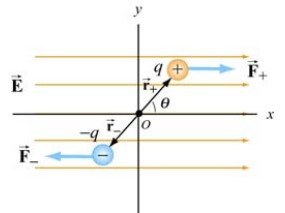
\includegraphics[width=8cm]{images/dipole_in_e_field.jpg}
\end{figure}

When an electric dipole is placed in a uniform external electric field $\vb{E}$ and makes angle $\theta$ with the field, torque $\tau$ is produced.

Torque $\tau$ is the cross product of vectors $\vb{p}$ and $\vb{E}$.
\begin{equation}
{\tau = \vb{p} \times \vb{E}
}\end{equation}

Magnitude of torque is given by
\[ \tau = pE\sin\theta \]



\subsection{Potential Energy of an Electric Dipole}


\pagebreak

\chapter{Magnetic Fields}
Magnetic B-field; Lorentz force; Ampère’s force; Biot-Savart law and B-field on the axis of a circular current loop and for simple symmetric systems like straight wire, circular loop and long solenoid.



\section{Magnetic Field}
Magnetic fields (or ``B" fields) are be created by magnetic dipoles. Just like electric charges are described as positive and negative charges, magnetic poles are described as north and south poles.\footnote{A magnetic monopole has never been found. This does not mean magnetic monopoles do not exist. We cannot prove magnetic monopoles do not exist; we can only say we have no evidence that they exist.}

A permanent magnet produces a special field around the magnet in which magnetic forces act. This field is called a \textbf{magnetic field} whose direction is the N-pole direction of a compass. 

An electric current produces a magnetic field that points clockwise around the current. If a current flows through a solenoid, a magnetic field that passes through the solenoid and points in the rightward direction is produced. 

The curves drawn to represent a magnetic field are called \textbf{magnetic field lines}. Magnetic field lines point outward from the N-pole of a permanent magnet and point inward to the S-pole; they neither disappear nor intersect one another.

Just like materials have an electric permittivity $\varepsilon$, materials also have a magnetic permeability $\mu$. Magnetic permeability is the measurement of the amount of magnetisation a material has in response to an external magnetic field. Magnetic permeability of free space has a constant value $\mu_0 = 4\pi \times 10^{-7}$ \unit{T.m.A^{-1}}.


\section{Magnetic Force on Current}
A magnetic field exerts a force on a current. If the magnetic field is in the direction of the index finger of a left hand and the current is in the direction of the middle finger, then the force on the current is in the direction of the thumb. This rule is called \textbf{Fleming’s left-hand rule}.

\begin{figure}[H]
    \centering
    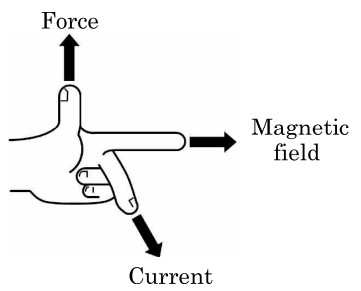
\includegraphics[width=8cm]{images/fleming_lhr.jpg}
\end{figure}

A magnetic field is defined by the fact that a moving electric charge in a B field can experience a magnetic force, $\vb{F}_B$.
\begin{equation}
{\vb{F}_B = 
}\end{equation}

\section{Electromagnetic Induction}
\textbf{Electromagnetic induction} is a phenomenon where an e.m.f. is induced when the number of magnetic field lines through the coil vary with time. The emf is induced to prevent the change in the magnetic field lines through the coil, and its magnitude is proportional to the instantaneous rate of change of the magnetic field lines through the coil.

\begin{thrm}{Biot-Savart law}{}
Magnetic field due to a long straight wire is
\begin{equation}
{B=\frac{\mu_{0} N I}{2 R}
}\end{equation}
\end{thrm}

\section{Ampere's Law}
We consider a straight conductor carrying a current of $I$. The magnitude of the magnetic field, $B$, on the circumference of radius $r$ in a plane perpendicular to the conductor is
\[ B \cdot 2\pi r = \mu_0I. \]
That is, the product of the length of the circumference and $B$ is equal to $\mu_0I$.




\begin{thrm}{Amp\`{e}re's law}{}
Line integral of $\vb{B}\cdot\dd{\vb{s}}$ around any closed path equals to $\mu_0I$, where $I$ is the total current passing through any surface bounded by the closed path:
\begin{equation}
{\oint \vb{B}\cdot\dd{\vb{s}} = \mu_0I}
\end{equation}
\end{thrm}

\begin{exmp}
A long straight wire of radius $R$ carries a steady current $I$ that is uniformly distributed through the cross-section of the wire.

Calculate the magnetic field at a distance $r$ from the centre of the wire in the regions $r\ge R$ and $r\le R$.
\end{exmp}

\section{Lorentz force}
In a uniform magnetic field of magnitude $B$, the magnitude of the magnetic force, $F$, that acts on a point charge of $q$ moving perpendicularly to the magnetic field at a speed of $v$ is
\[ F=Bqv \]



\section{Electromagnetic Induction and Self-Inductance}

\section{}


Gauss’ law (for E- and B-fields); Ampère’s law; Faraday’s law; using these laws for the calculation of fields when the integrand is almost piece-wise constant. 

Boundary conditions for the electric field (or electrostatic potential) at the surface of conductors and at infinity; concept of grounded conductors. 
Superposition principle for electric and magnetic fields; uniqueness of solution to well-posed problems; method of image charges.
\pagebreak

\chapter{Interaction of matter with electric and magnetic fields}
Resistivity and conductivity; differential form of Ohm’s law. 
Dielectric and magnetic permeability; relative permittivity and permeability of electric and magnetic materials; energy density of electric and magnetic fields; ferromagnetic materials; hysteresis and dissipation; eddy currents; Lenz’s law. 
Charges in magnetic field: helicoidal motion, cyclotron frequency, drift in crossed E- and B-fields. 
Energy of a magnetic dipole in a magnetic field; dipole moment of a current loop.
\pagebreak

\chapter{Circuits}
Linear resistors and Ohm’s law; Joule’s law; work done
by an electromotive force; ideal and non-ideal batter-
ies, constant current sources, ammeters, voltmeters and
ohmmeters. Nonlinear elements of given V -I characteristic. 

\chapter{Capacitors and Inductors}
\section{Capacitance and inductance}
\textbf{Capacitors} are used to store energy in electrical and electronic circuits. 

Every capacitor has two leads, each connected to a metal plate. To store energy, these two plates must be given equal and opposite electric charges. Between the plates is an insulating material called the \textbf{dielectric}.

Applying a potential difference to the plates of a capacitor causes electrons to move to or from the plates. Electrons are removed from one plate, and an equal number of electrons are added to the other plate.

\begin{figure}[H]
    \centering
    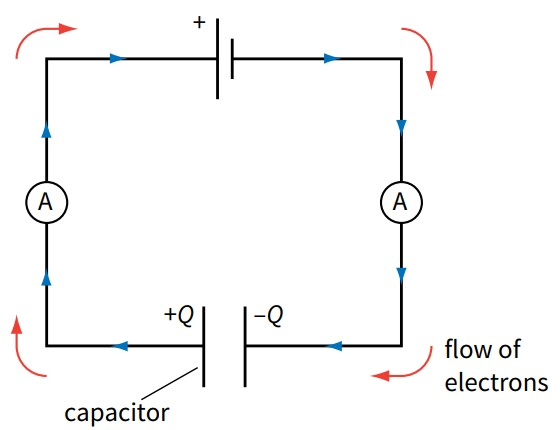
\includegraphics[width=8cm]{images/capacitor.jpg}
\end{figure}

\begin{defn}{Capacitance}{}
Ratio of the change in electric charge on either conductor of a capacitor to the change in potential difference between them.
\begin{equation}
{C \equiv \frac{Q}{V}
}\end{equation}
\end{defn}

\[ C=k\varepsilon_0\frac{A}{d} \]
where $k$ depends on the material between the plates.

An \textbf{inductor} is a passive component used to store energy in the form of magnetic energy when electricity is applied to it. One of the key properties of an inductor is that it impedes or opposes any change in the amount of current flowing through it.

\begin{defn}{Self-inductance}{}
Ratio of the e.m.f. induced in an electrical circuit or component to the rate of change of current causing it.
\[ V = L \dv{I}{t} \]
\end{defn}

\begin{defn}{Mutual inductance}{}
Tendency of an electrical circuit or component to oppose a change in the current in a nearby electrical circuit or component.
\end{defn}

\section{Dielectrics and ferromagnetic materials}
\begin{defn}{Dielectric material}{}
Dielectric materials enhance capacitance by allowing the electric field between the plates to induce charge dipoles in it, thus increasing the ability of the capacitor to store energy; dielectric breakdown can occur when the electric field is sufficiently strong, where a conducting path between the plates is formed and charge jumps across the gap, usually destroying the capacitor.
\end{defn}

\begin{defn}{Ferromagnetic material}{}
Ferromagnetic materials enhance inductance by allowing the magnetic field within the inductor to align its domains, thus increasing the ability of the inductor to store energy; this enhancement is non-linear as the magnetic field due to the current increases, especially near saturation where the intrinsic magnetic dipole moments within the material are almost aligned perfectly with the field and cannot be further aligned to produce still higher magnetisation.
\end{defn}

\section{Energy in a capacitor and in an inductor}
\begin{figure}[H]
    \centering
    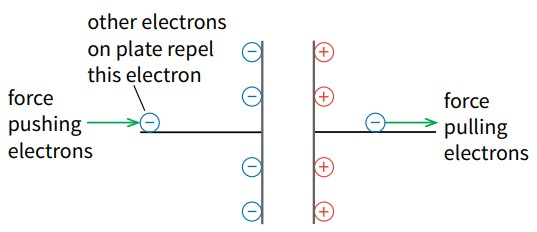
\includegraphics[width=8cm]{images/capacitor_energy.jpg}
\end{figure}

Energy stored in capacitor:
\begin{equation}
{U = \frac{1}{2}CV^2 = \frac{1}{2}QV
}\end{equation}

\begin{proof}
Potential energy stored in a capacitor $U$ is equal to the work done $W$ by a battery with potential difference $V$ to put a charge $Q$ on a capacitor with capacitance $C$.

Work done on a charge against an element of potential difference in the battery is given by $\dd{W} = Q \dd{V}$.

From the definition of capacitance, 
\[ C = \frac{Q}{V} \implies Q = CV \]

Thus 
\[ \dd{U} = \dd{W} = Q \dd{V} \implies U = \int_0^V CV \dd{V} = \frac{1}{2}CV^2 \]
\end{proof}

Potential energy stored in an inductor is 
\begin{equation}
{U = \frac{1}{2}LI^2
}\end{equation}

\begin{proof}
The potential energy stored in an inductor $U$ is equal to the work done $W$ by a battery to move a charge $Q$ through the inductor.

Work done on an element of charge against the potential difference in a battery is $\dd{W} = V \dd{Q}$.

From the definition of inductance, \[ V = L \dv{T}{t} \]

Thus 
\[ \dd{U} = \dd{W} = L\dv{I}{t}\dd{Q} = LI\dv{Q}{t} \dd{I} \implies U = \int_0^I LI \dd{I} = \frac{1}{2}LI^2 \]
\end{proof}


\section{Circuits with capacitors and inductors}
Capacitors arranged in series: (common charge on capacitors)
\[ \frac{1}{C_T} = \sum_i\frac{1}{C_i} \]

Capacitors arranged in parallel: (common p.d. across capacitors)
\[ C_T = \sum_iC_i \]

Inductors in series (common rate of change of current through inductors)
\[ L_T = \sum_iL_i \]

Inductors in parallel (common self-induced e.m.f. across inductors)
\[ \frac{1}{L_T} = \sum_i\frac{1}{L_i} \]





Capacitors and capacitance (also for a single electrode with respect to infinity); self-induction and inductance; energy of capacitors and inductors; mutual inductance; time constants for RL and RC circuits. 

\chapter{Inductors}


\chapter{AC circuits}
AC
circuits: complex amplitude; impedance of resistors, in-
ductors, capacitors, and combination circuits; phasor di-
agrams; current and voltage resonance; active power.

